\begin{table}[h]
    \centering
    \begin{tabular}{lllr}
    \toprule
    \textbf{feature} 
        & \textbf{type}
        & \textbf{description}
        & \textbf{NA}
        \\
    \midrule
    sex 
        & \texttt{fct(2)}
        & demographical
        & 0
        \\ 
    \midrule
    chest.pain 
        & \texttt{fct(4)}
        & clinical
        & 0
        \\
    \midrule
    fbs 
        & \texttt{fct(2)}
        & clinical
        & 0
        \\
    \midrule
    rest.ecg 
        & \texttt{fct(3)}
        & clinical
        & 0
        \\
    \midrule
    angina 
        & \texttt{fct(2)}
        & clinical
        & 0
        \\
    \midrule
    blood.disorder 
        & \texttt{fct(3)}
        & clinical
        & {\color{red} 2}
        \\
    \midrule
    age 
        & \texttt{int}
        & demographical
        & 0
        \\
    \midrule
    bp 
        & \texttt{int}
        & clinical
        & 0
        \\
    \midrule
    chol 
        & \texttt{int}
        & clinical
        & 0
        \\
    \midrule
    heart.rate 
        & \texttt{int}
        & clinical
        & 0
        \\
    \midrule
    vessels 
        % & \texttt{\color{red} int/fct(4)}
        & \texttt{int}
        & clinical
        & 0

        \\
    \midrule
    st.depression 
        & \texttt{dbl}
        & clinical
        & 0
        \\
    \bottomrule
    \toprule
    \textbf{response} 
        & \textbf{type}
        & \textbf{value}
        & \textbf{count}
        \\
    \midrule
    \multirow{2}{*}{disease}
        & \multirow{2}{*}{\texttt{fct(2)}}
        & 0 (absence) & 138*
        \\
        && 1 (presence) & 162*
        \\
    \bottomrule
\end{tabular}
    
    \raggedleft {\tiny (*) before NA exclusion}
    
    \vspace{4pt}
    \caption{Dataset features}
\end{table}

\section{Exploratory Data Analysis}


\subsection{Description of dataset}
The dataset comprises of \( 300 \) raw records and \( 12 \) different features. Although the data is already cleaned, there are 2 records with \( \texttt{blood.disorder} = 0 \), noting that no data was recorded in this field. We will simply remove these \( 2 \) records from our dataset.

\begin{table}[H]
    \centering
    \begin{tabular}{rrrrrr}
        \hline
        \textbf{Value} & 0 & 1 & 2 & 3 & Total\\
        \hline
        \textbf{Frequency} & 2 & 18 & 163 & 117 & \(n = 300\)\\
        \hline
    \end{tabular}
    \vspace{4pt}
    \caption{Frequency table of \texttt{blood.disorder}}
\end{table}


% \textbf{The \texttt{vessels} variable}. Despite being an integral feature, it only ranges from 0 to 4. For our purposes, we will consider \texttt{vessels} as a categorical variable of 5 factors \( \{0, 1, 2, 3, 4\} \).




\subsection{Categorical variables}
There are 6 categorical variables in the dataset, 5 of which are different types of clinical metrics 
(\texttt{angina}, \texttt{blood.disorder}, \texttt{chest.pain}, \texttt{fbs}, \texttt{rest.ecg}). In general, there is a disproportionate ratio of categories within the dataset. For example,
\begin{itemize}
    \item There are \textit{twice} the number of patients who experienced angina induced by exercise (\texttt{angina = 0}) compared to those that did not (\texttt{angina = 1});
    \item The number of patients having high fasting blood sugar level (\texttt{fbs = 1}) is about \textit{five times lower} than those having low fasting blood sugar level (\texttt{fbs = 0}).
\end{itemize}

\begin{figure}[h]
    \centering
    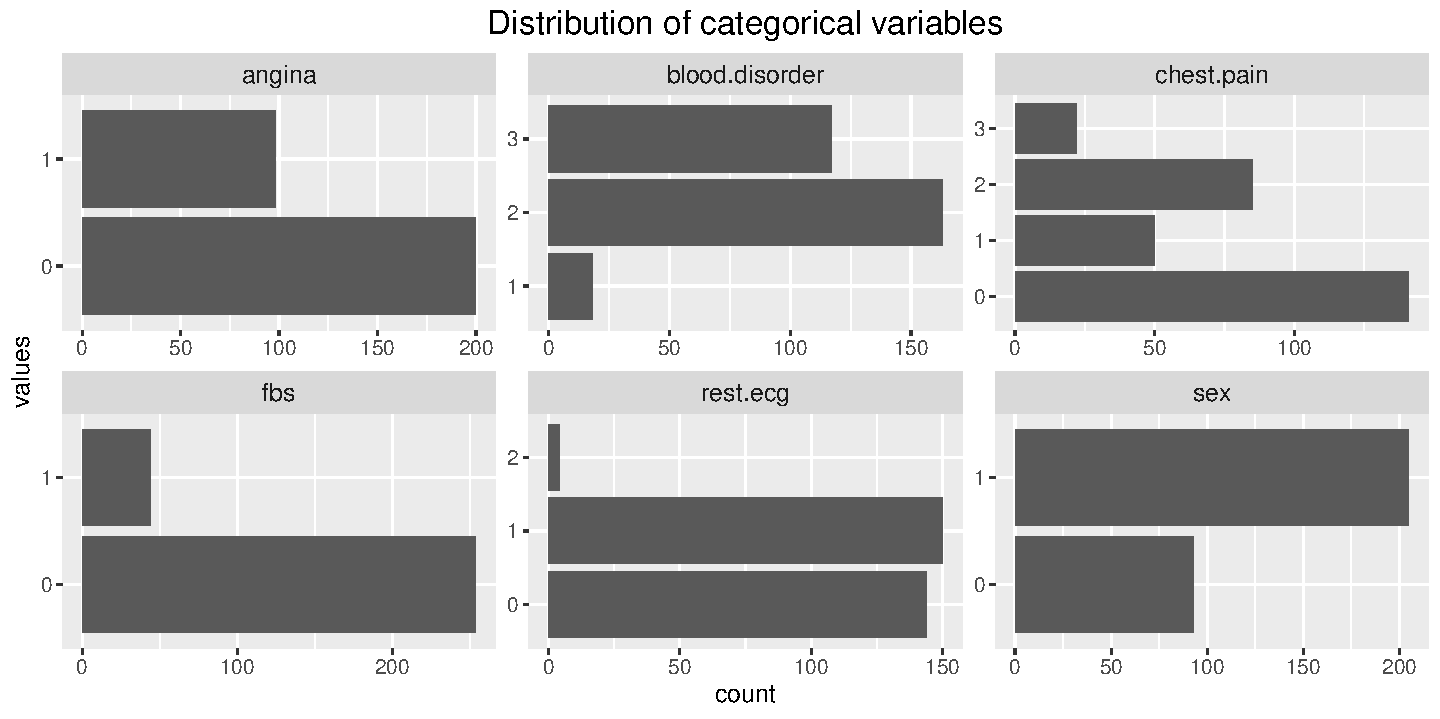
\includegraphics[width=\linewidth]{22.categorical.distribution.pdf}
    \caption{\centering Distribution of categorical variables}
\end{figure}

To test the significance of these features in predicting the presence of disease, two methods are used: \textit{percent stacked bar chart} and \textit{Fisher's exact test}. For a graphical inference, conditional probabilities \( \mathbb P[Y = y | X_i = x_i] \) (\( X_i \) being a categorical feature) are calculated and plotted on a \textit{percent stacked bar chart}. By visual inspection, it can be seen that the level of fasting blood sugar (\texttt{fbs}) is weakly correlated to the presence of disease. 

\begin{figure}[h]
    \centering
    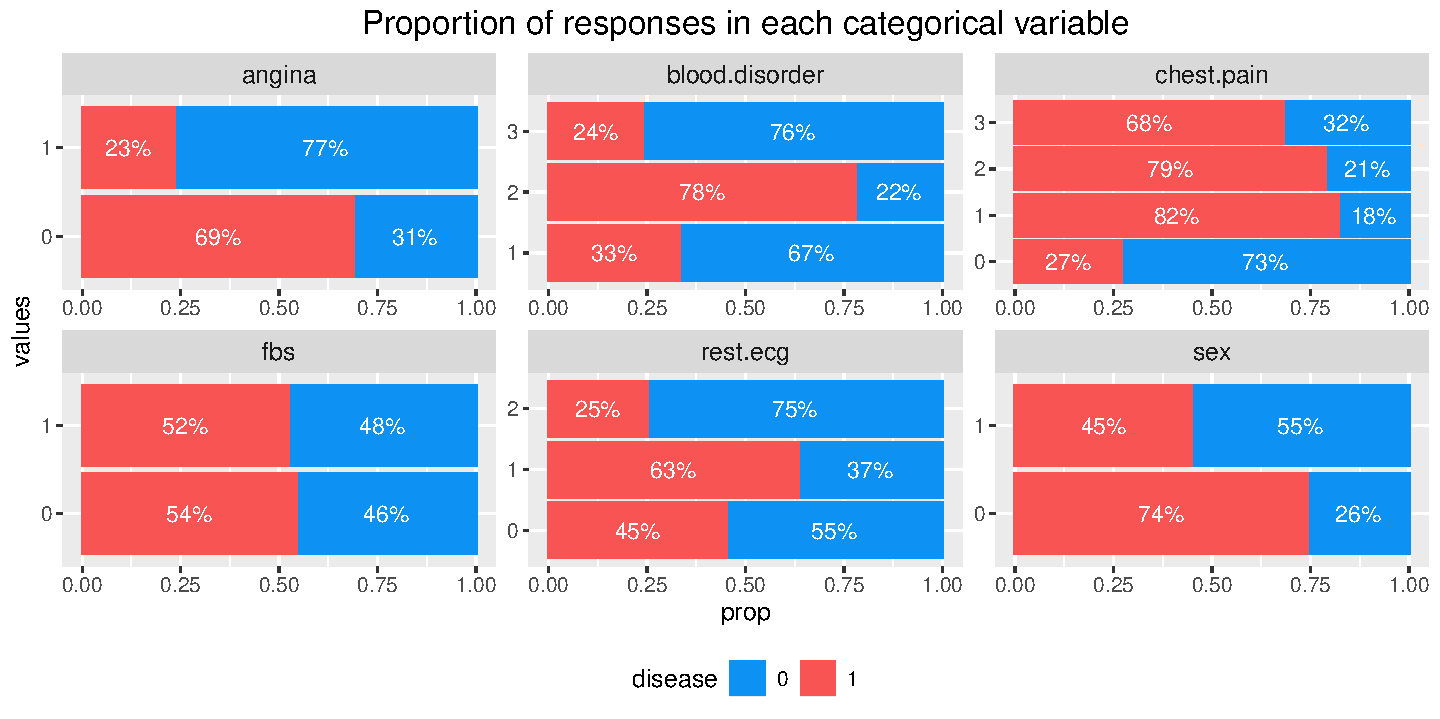
\includegraphics[width=\linewidth]{22.categorical.correlation.to.response.pdf}
    \caption{\centering Relationship of categorical features to the response variable}
\end{figure}

Indeed, one can calculate the odds ratio as
\begin{align*}
    \mathrm{OR} 
    &= 
    \frac{\mathbb P[Y = 1 | X = 1]}{\mathbb P[Y = 1 | X = 0]}\cdot
    \frac{\mathbb P[Y = 0 | X = 0]}{\mathbb P[Y = 0 | X = 1]}
    \\
    &\approx
    \frac{52\% \cdot 46\%}{54\% \cdot 48\%}
    \approx
    0.92
\end{align*}
which may suggests an insignificant correlation between fasting blood sugar and the presence of disease.

For a quantitative contigency test, \textit{Fisher's exact test} \citep{fishertest} is used. From applying Fisher's test, it is observed that there are
\begin{itemize}
    \item \textbf{No evidence of correlation} between the presence of disease and the categorical level of fasting blood sugar ($p > 10^{-2}$).
    \item \textbf{Correlation} between the presence of disease and other clinical measures ($p < 10^{-4}$).
\end{itemize}

\begin{table}[h]
    \centering
    \begin{tabular}{lr}
        \toprule
        \textbf{Variable} & \textbf{Fisher's p-value}\\
        \midrule
        angina          & $<$ 0.0001\\
        \midrule
        blood.disorder  & $<$ 0.0001\\
        \midrule
        chest.pain      & $<$ 0.0001\\
        \midrule
        \color{red}{fbs}        & \color{red}{0.8703}\\
        \midrule
        \color{gray}{rest.ecg}  & 0.0019\\
        \midrule
        sex             & $<$ 0.0001\\
        \bottomrule
    \end{tabular}
    
    \vspace{4pt}
    \caption{\centering Fisher's $p$-value for categorical variables}
\end{table}


\subsection{Numerical variables}
\begin{figure}[h]
    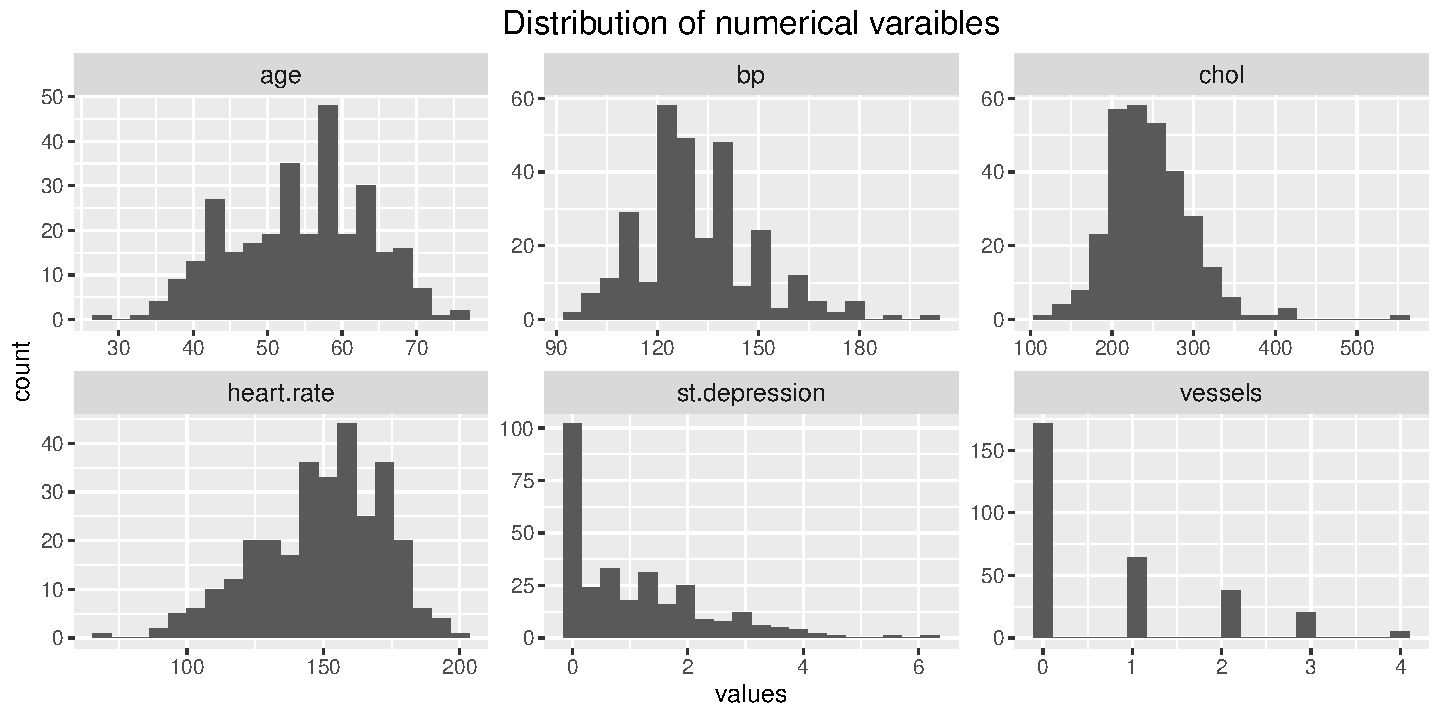
\includegraphics[width=\linewidth]{23.numerical.distribution.pdf}
    \caption{\centering Histogram of numerical features}
\end{figure}

There are 6 numerical variables in the dataset, 5 of which are different types of clinical metrics 
(\texttt{bp}, \texttt{chol}, \texttt{heart.rate}, \texttt{st.depression}, \texttt{vessels}). In general, by plotting the histograms for the variables, it is observed that some of the features (\texttt{bp}, \texttt{heart.rate}, \texttt{chol}) are 'close' to a normal distribution, whilst others are heavily \textit{left-skewed} (\texttt{age}) or \textit{right-skewed} (\texttt{st.depression}, \texttt{vessels}).


The relationship of number variables and the response is tested on a faceted box-plot. By visually comparing the distribution mean of each group, it can be seen that there are 

\begin{itemize}
    \item \textbf{Strong correlation} between varibles \texttt{age}, \texttt{heart.rate}, \texttt{vessels}, \texttt{st.depression} and the response variable;
    \item \textbf{Weak correlation} between \texttt{bp} and \texttt{chol} and the response variable
\end{itemize}

\begin{figure}[h]
    \centering
    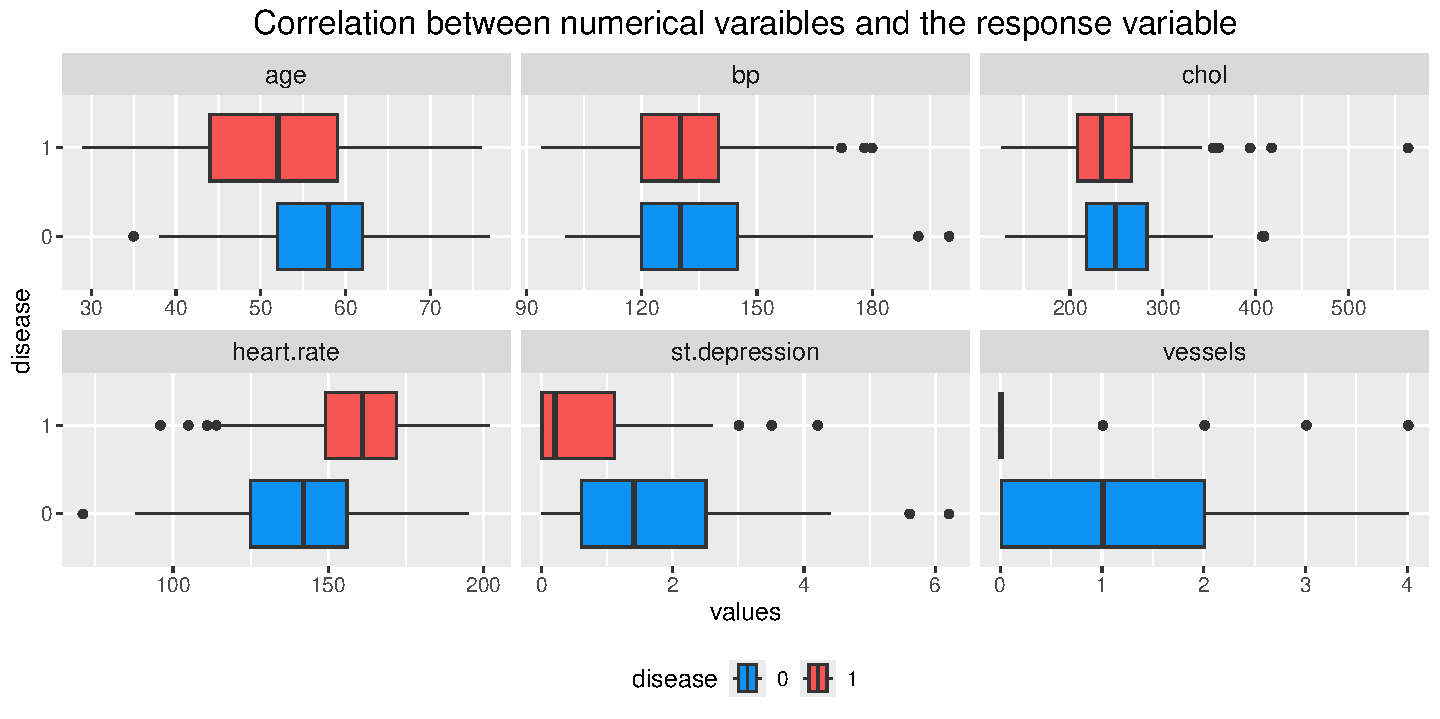
\includegraphics[width=\linewidth]{23.numerical.correlation.to.response.pdf}
    \caption{\centering Boxplot correlation with disease}
\end{figure}

To test for normality for each variables, a QQ-plot is used for visualisation, along with the p-value from the \textit{Shapiro-Wilk normality test} \citep{shapirotest}. As no variables are normally distributed (all \( p < 10^{-2} \)), normality transformations are also considered. In this case, the transformation of interest is the \textit{Box-Cox transformation}, a parametric transformation that generalises power and logarithmic transformations on positive variables with a single parameter \( \lambda \):

\[
    B_\lambda(x) = \begin{cases}
        \frac{x^\lambda - 1}{\lambda}   & \text{if \( \lambda \ne 0 \)} \\
        \ln{x}                          & \text{if \( \lambda  =  0 \)}
    \end{cases}
\]

For non-negative variables, a \( x \mapsto x + \varepsilon \) transformation, where \( \varepsilon = 0.01\), is applied before Box-Cox to prevent the transformation being undefined at \( x = 0 \).

Different values of \( \lambda \) in the range \( [-5, 5] \) are tested, the value of which yields the best \textit{Shapiro-Wilk's p-value} is retained. It can be observed that \texttt{age}, \texttt{bp}, \texttt{chol} and \texttt{heart.rate} are Box-Cox transformable to a normally distributed variable, within a \( 99\% \) level of significance. In contrast, heavy right-skewed variables (\texttt{st.depression} and \texttt{vessels}) fail to be normally transformable by the Box-Cox transformation.

\begin{figure}[h]
    \centering
    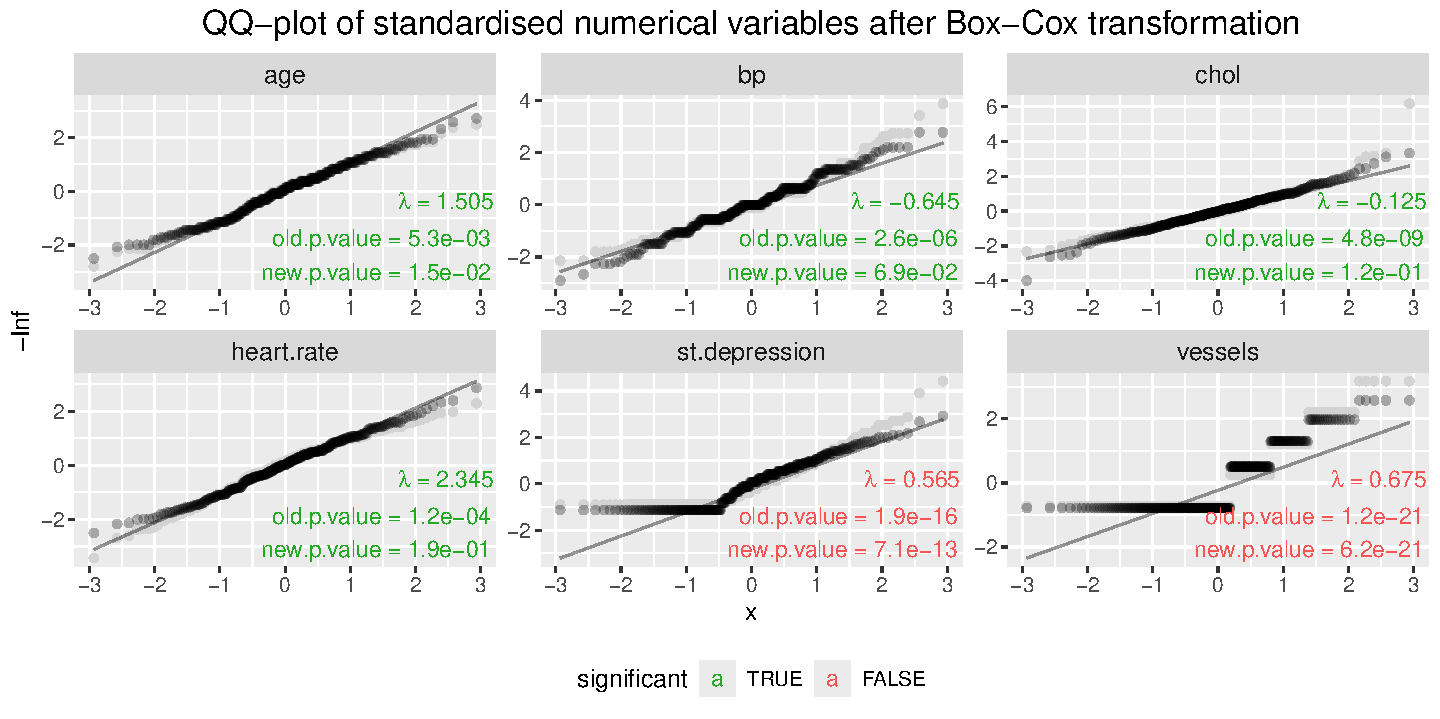
\includegraphics[width=\linewidth]{23.numerical.boxcox.qq.pdf}
    \caption{\centering Best Box-Cox transformation for each numerical variable}
\end{figure}



\subsection{Conclusion}
The dataset is a cleaned, 300-record dataset that shows the relationship between demographical and clinical features and the presence of heart disease. A combination of numerical and categorical variables are featured in this dataset, and whilst most features have strong correlation with the response variable, some features seem to be a weak predictor to heart disease (such as \texttt{fbs}, \texttt{bp} or \texttt{chol}). In further sections, models with or without this set of features will be tested against each other.